% !TEX root = ../main.tex
\documentclass[../main.tex]{subfiles}
\begin{document}

\subsection{Disk, Bulge and Bar}

After having obtained aggregated models for our galaxies, we need to validate the reliability of our models through comparison to other results in the literature. The comparisons we will make are listed below:

\begin{itemize}
    \item Comparison of Disk axial ratio to NSA photometry
    \item Comparison of frequency of drawn bulges or bars to GZ2 morphology
    \item Comparison of aggregated bulge size to GZ2 vote fraction
    \item Comparison of aggregated bar length to GZ2 and photometrically fitted bars
\end{itemize}

For instance, if we compare the axis ratios of the disks recovered from galaxy builder to the axis ratio of a 2D S\'ersic fit to the r-band SDSS image of each galaxy (as provided in the NASA-Sloan Atlas), we see good agreement (Fig.\ref{fig:ax_ratio_comparison})

\begin{figure}
  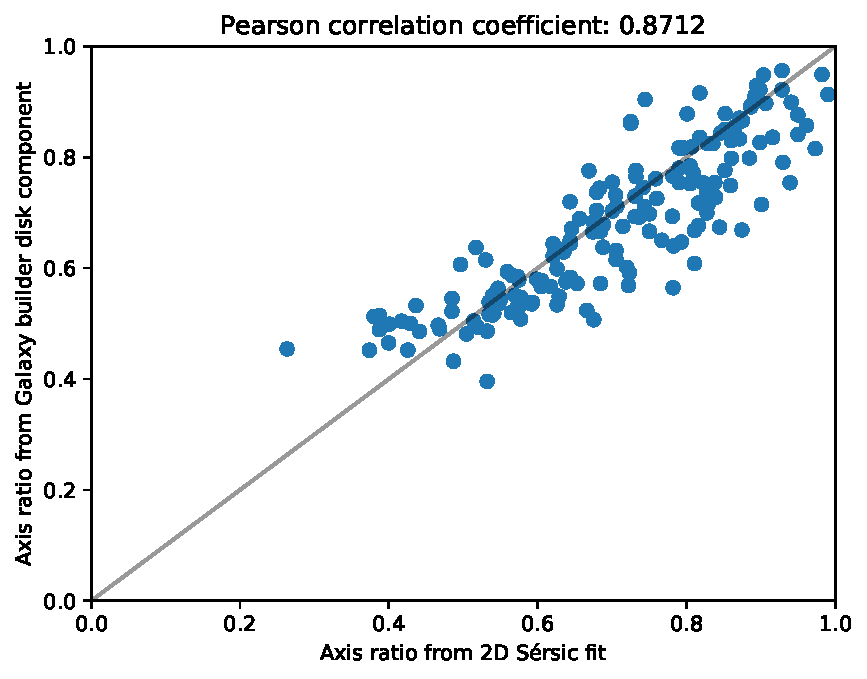
\includegraphics[width=8cm]{images__results/GZBvsNSA_ax-ratio_SERSIC_BA.pdf}
  \caption{Comparison between the axis ratios of the disk components of aggregated Galaxy Builder models to the results of an r-band S\'ersic profile fit.}
  \label{fig:ax_ratio_comparison}
\end{figure}

We can also make comparisons to existing measures of morphology for individual galaxies. For instance, using GZ2 results, we can investigate how likely a volunteer is to incorporate a bulge or bar component in their model relative to its existing morphological classification obtained by citizen scientists.

Mirroring \citet{Kruk2017:1710.00093v2}, we define a galaxy as disk dominated if the debiased GZ2 fractions $p_\text{no bulge} + p_\text{just noticeable} > p_\text{obvious bulge} + p_\text{dominant bulge}$, or bulge dominated if the converse. Grouping our galaxies based on their type results in no significant difference in the probability of bulge being present in their model. The probability of a classification of a disk dominated galaxy having a bulge was \comment{$0.7293 \pm 0.0781$}, whereas for a bulge dominated galaxy it was \comment{$0.7707 \pm 0.0806$}.

However, when comparing the probability of a classification containing a bar component against a galaxy being classed as strongly-barred or as having no bar (as defined in \citealt{Masters2010:1003.0449v2}), we see a significant difference: classifications of strongly-barred galaxies ($p_\text{bar} > 0.5$) had a \comment{$0.5713 \pm 0.1549 \%$} of containing a bar, vs \comment{$0.3666 \pm 0.1147\%$} for galaxies classed as having no bar ($p_\text{bar} < 0.2$). A T-test returns the probability of the two samples being the same as less than \comment{$0.0002\%$}. Disregarding the bar / no bar classifications, the Spearman correlation between GZ2's $p_\text{bar}$ and the bar likelihood in galaxy builder is \comment{$0.751$}.


% \comment{Compare bulge / disk ratio?}

% \comment{Pbar vs number of bars drawn}

% \comment{Pspiral vs frequency of classification having spiral arms}


\subsection{Spiral Arms}

In order to benchmark the reliability of this method of spiral parameter extraction, we compare the result of our logarithmic spiral fit to the relationship obtained by \citet{Hart2016:1607.01019v1} between GZ2 classification and galaxy pitch angle (Fig.\ref{fig:hart_pitch_angle}). We find good agreement, though the large error bars on the GZ2-produced pitch angle (along with the caveat in the paper that these pitch angles should not be used for individual galaxies) make this comparison rather inconclusive.

The fit obtained by \citet{Hart2016:1607.01019v1} was obtained by using a leading automated spiral arm detection and fitting tool, \textsc{SpArcFiRe} \citep{Davis2014:1402.1910v1}.

points in each arm cluster to that produced by a leading automated spiral arm detection and fitting tool, \textsc{SpArcFiRe} \citep{Davis2014:1402.1910v1}.

\begin{figure}
  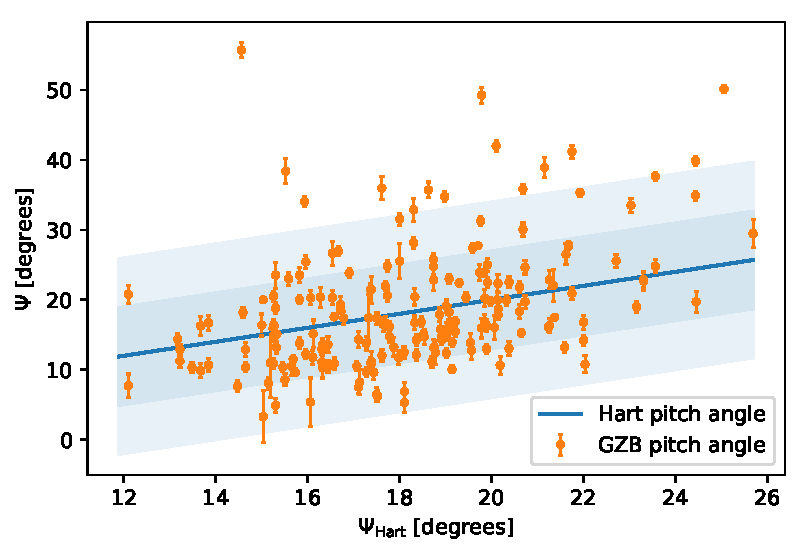
\includegraphics[width=8cm]{images__results/pitch-angle-comparison.pdf}
  \caption{A comparison of Pitch angle obtained by \citet{Hart2016:1607.01019v1} with measured pitch angles for the aggregated model results in galaxies in the Galaxy Zoo Builder sample}
  \label{fig:hart_pitch_angle}
\end{figure}


\comment{Show results of sparcfire / GZ2 comparison}

\subsubsection{Model selection}

\comment{This is more "Are log spirals right?", should it go in a different paper?}

Group K-fold cross validation is used to perform model selection, where points are grouped according to the poly-line they were drawn in. Five folds is chosen as a compromise to minimise variance on the resulting scores, while also minimising the bias from removing too many classifications from our training set. To score the goodness-of-fit of a model, we use negative median absolute error.


In order to confidently describe a spiral arm as not a logarithmic spiral, we \comment{TODO}

\end{document}
